\section{Security in AWS}

\textbf{Authors}: Sinchan Bangalore Sheshadri



One of AWS’s advantages is the availability of a wide variety of services. The smooth integration of different services due to their VPC makes it easy to integrate and deploy projects. As an added benefit, most of the security implementation can be easily implemented using their AWS Console.

In our security implementation, we have used several services such as Route 53, EC2 Load Balancers, AWS Certificates Manager (ACM), AWS Secrets Manager, and AWS Relational Database Service (RDS).


\subsection{Enabling Encrypted Communication}

AWS offers a multitude of services that aid in having a smooth development environment. For the task of enabling encrypted communication, we use the services of Route 53, ACM, and EC2 Load Balancer. The aim is to secure the communication line using HTTPS. The steps involved in establishing an HTTPS connection are as follows.

•	Register a domain in AWS Route 53

Route 53 allows us to register a domain of our choice subject to its availability. AWS offers the domains on a per-year renewal basis. Domains are priced differently based on the top-level domains (TLD).


•	Request a certificate from the AWS certificate manager (ACM)

The next step is to obtain the certificate for the TLS. ACM offers the ability to either request a certificate or import a certificate. The issued certificates are valid for one year.

The certificates issued by the ACM have the added advantage of auto-renewal. These certificates will automatically be renewed once it reaches its expiration.


•	Set up an HTTPS Listener on the Application Load Balancer in EC2 load balancers

The final step is to create an HTTPS listener on the load balancer to route traffic through the secured line. When creating this listener and adding rules, a certificate must be assigned. The ACM issued certificate is used here.

Once the load balancer is correctly set up with its security groups and VPC, the web application is now accessible over HTTPS.



In our approach, we obtained the domain ‘onlinedvdmovie.de’ from AWS Route 53. A certificate for the obtained domain can be issued with the help of ACM. The certificate issued for the domain obtained from Route 53 is eligible for auto-renewal.


\begin{figure}[h]
\centerline{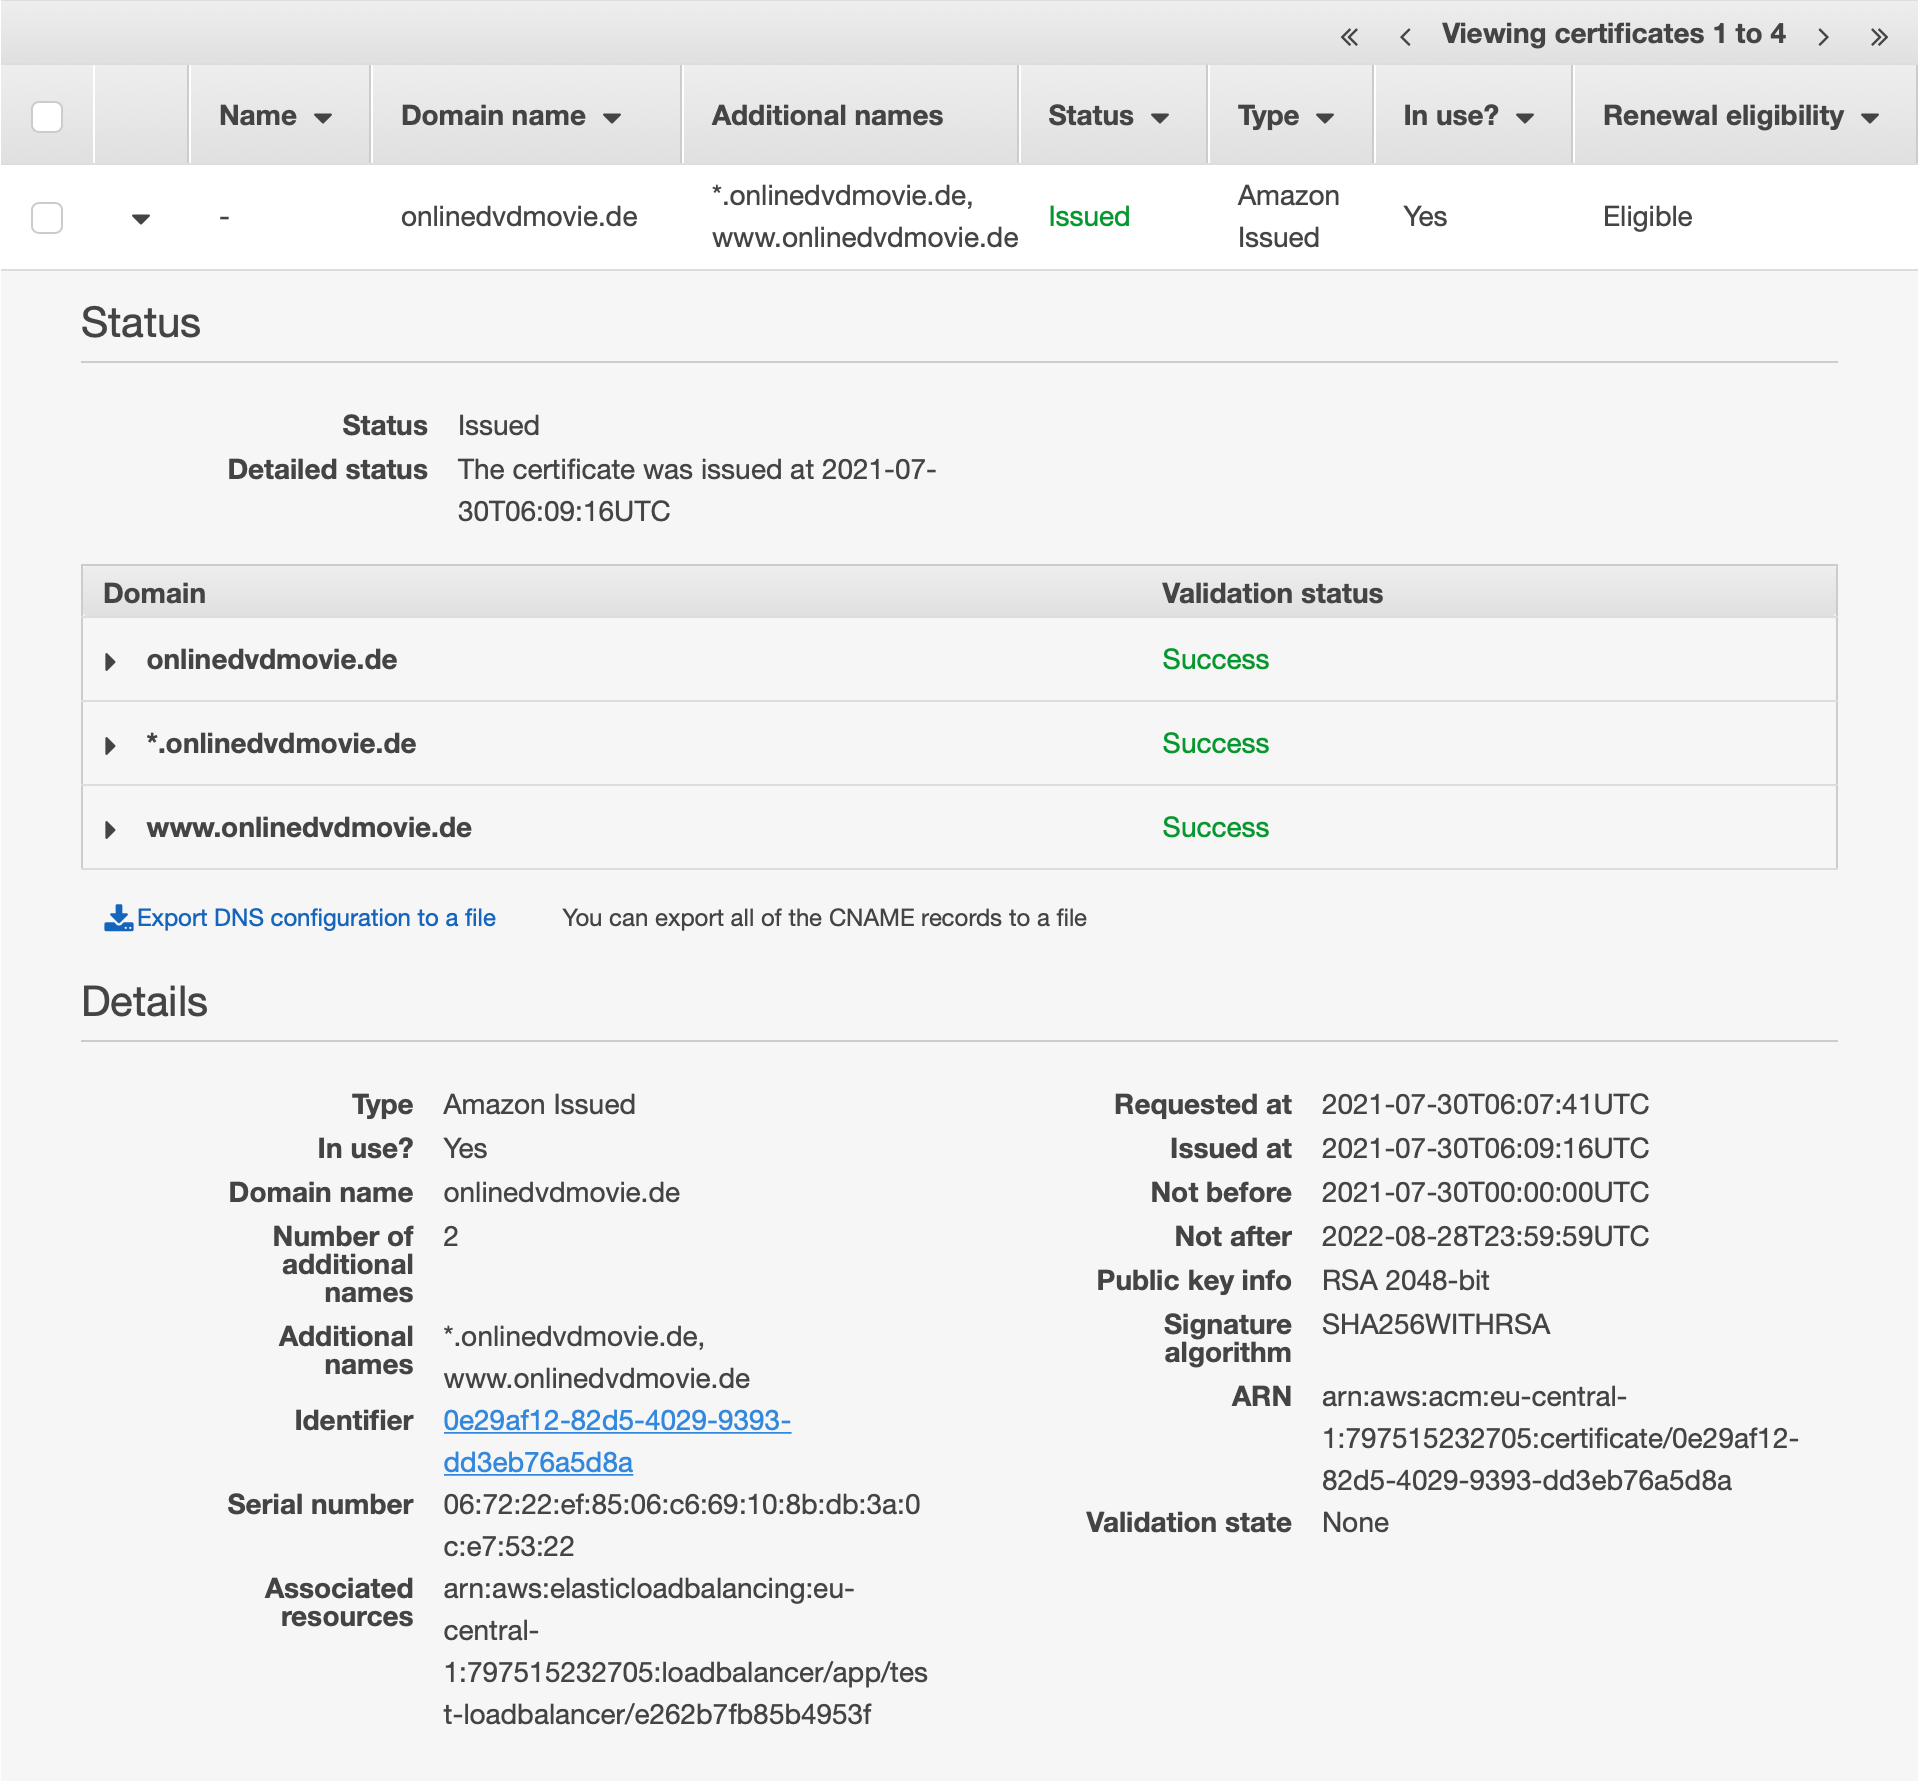
\includegraphics[scale=.50]{images/Sinchan/6sinchan.png}}
\caption{The certificate obtained for www.onlinedvdmovie.de}
\label{fig6sinchan}
\end{figure}

In the next step, we configure the traffic listeners on the application load balancer. As shown in \autoref{fig3sinchan}, an HTTP listener is set up at port 80 to redirect all incoming traffic to ‘https://onlinedvdmovie.de:443/?’ which is an HTTPS listener with port 443.


\begin{figure}[h]
\centerline{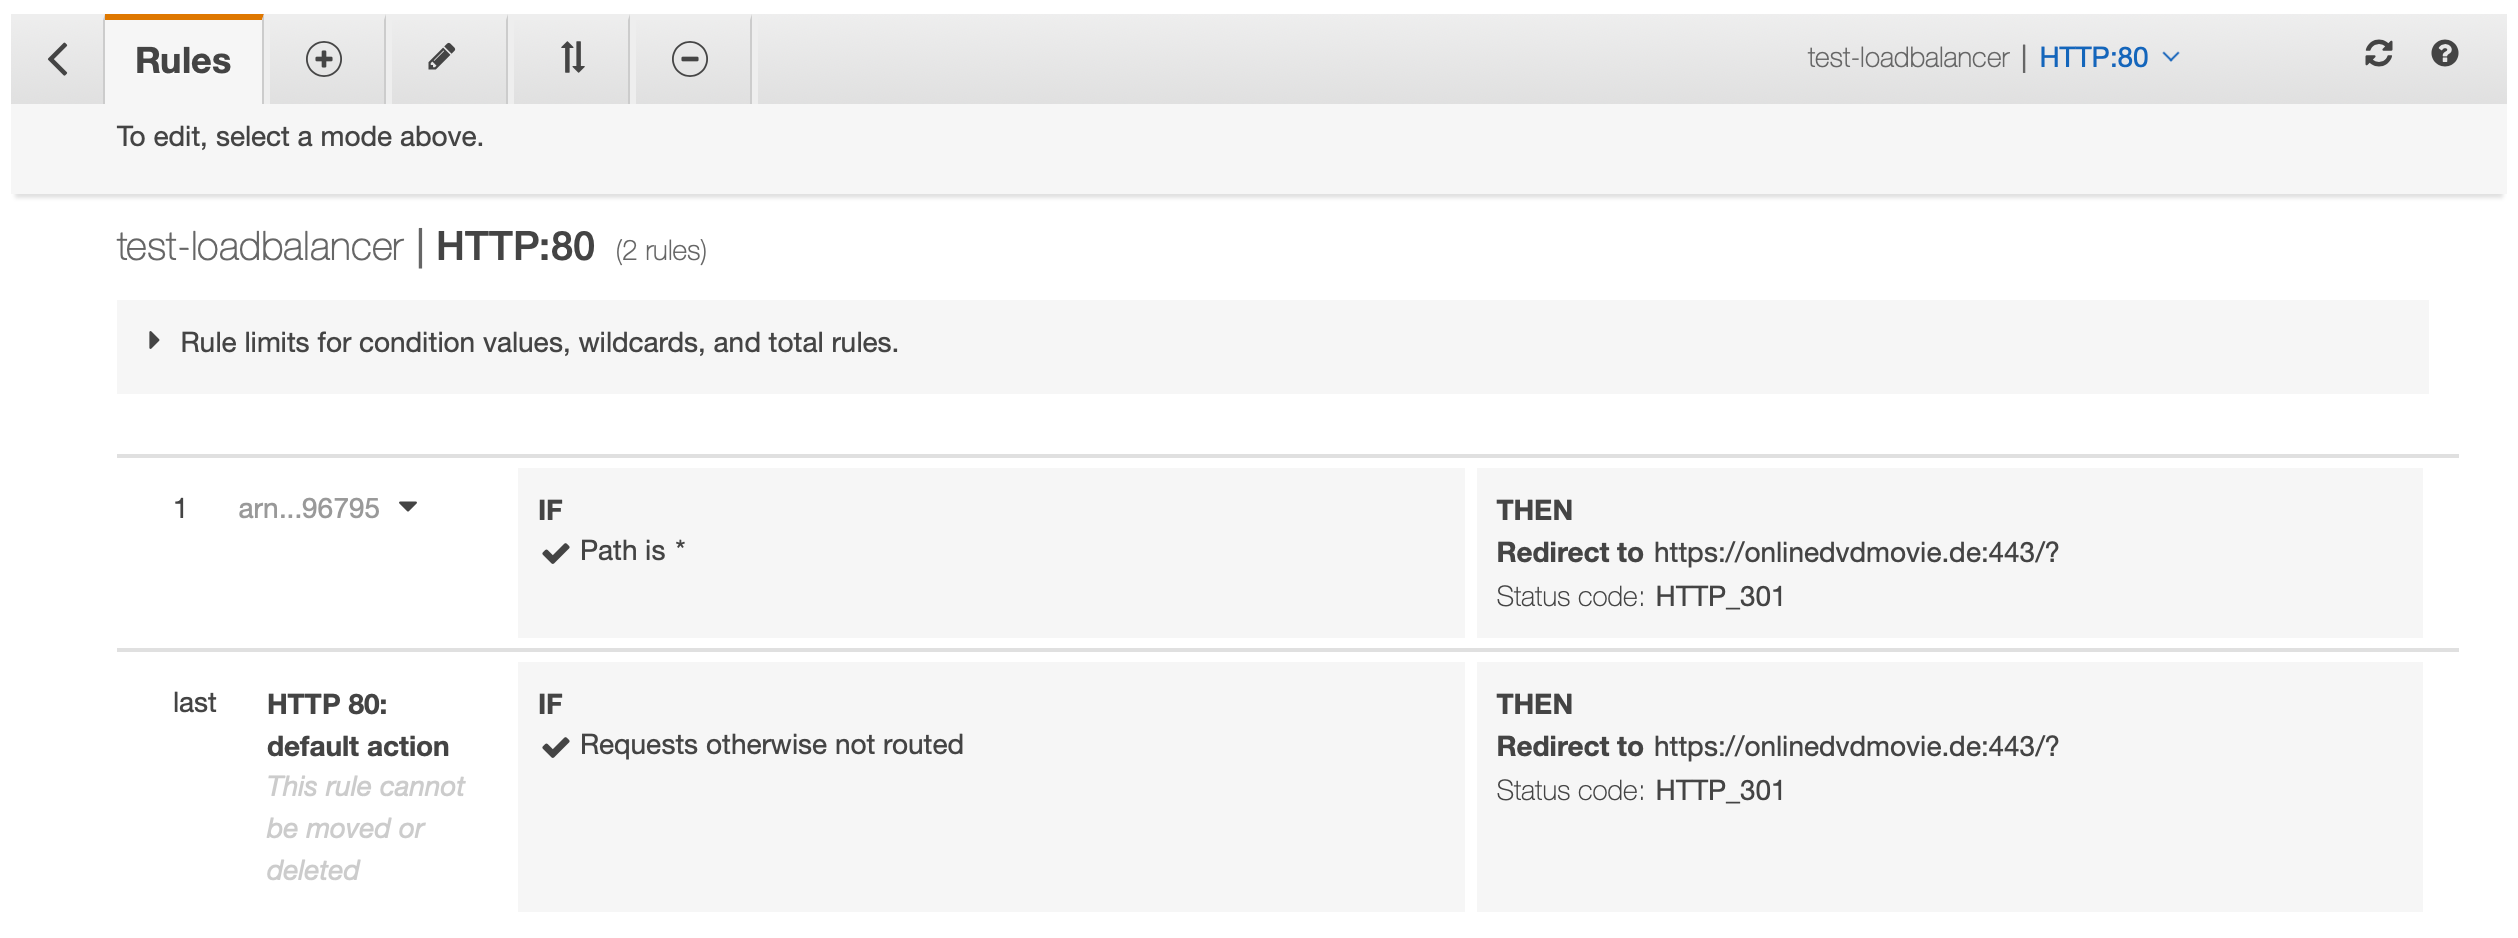
\includegraphics[scale=.38]{images/Sinchan/3sinchan.png}}
\caption{HTTP listeners set up on the load balancer}
\label{fig3sinchan}
\end{figure}



The HTTPS listener is configured to forward the incoming requests to the respective target group where the requests are served as seen in \autoref{fig1sinchan}

\begin{figure}[h]
\centerline{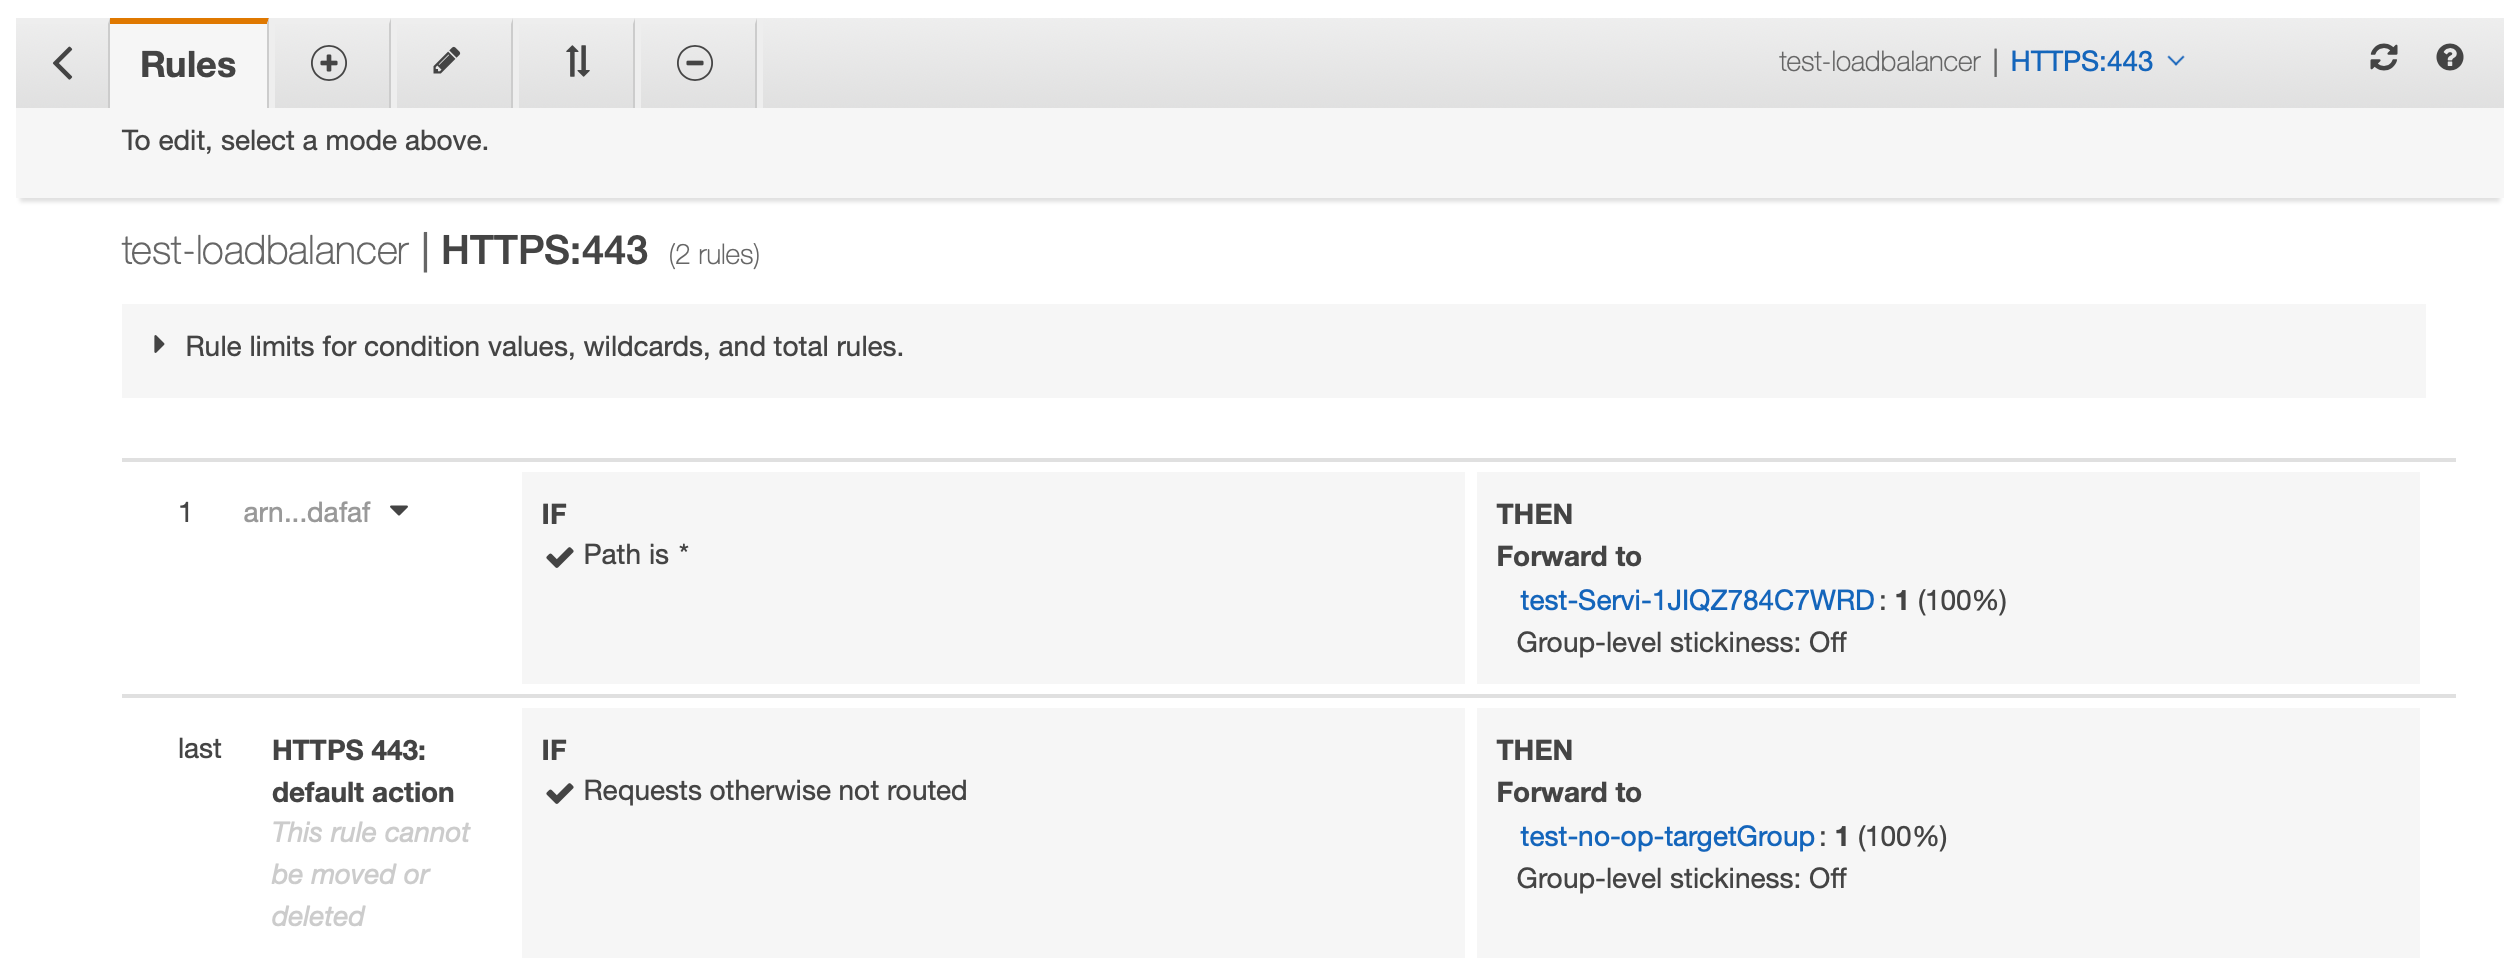
\includegraphics[scale=.36]{images/Sinchan/1sinchan.png}}
\caption{HTTPS listeners set up on the load balancer}
\label{fig1sinchan}
\end{figure}

With this, when we visit the domain ‘onlinedvdmovie.de’, we can see the associated certificate to the domain, confirming that the connection is secure as showin in \autoref{fig5sinchan}.

\begin{figure}[h]
\centerline{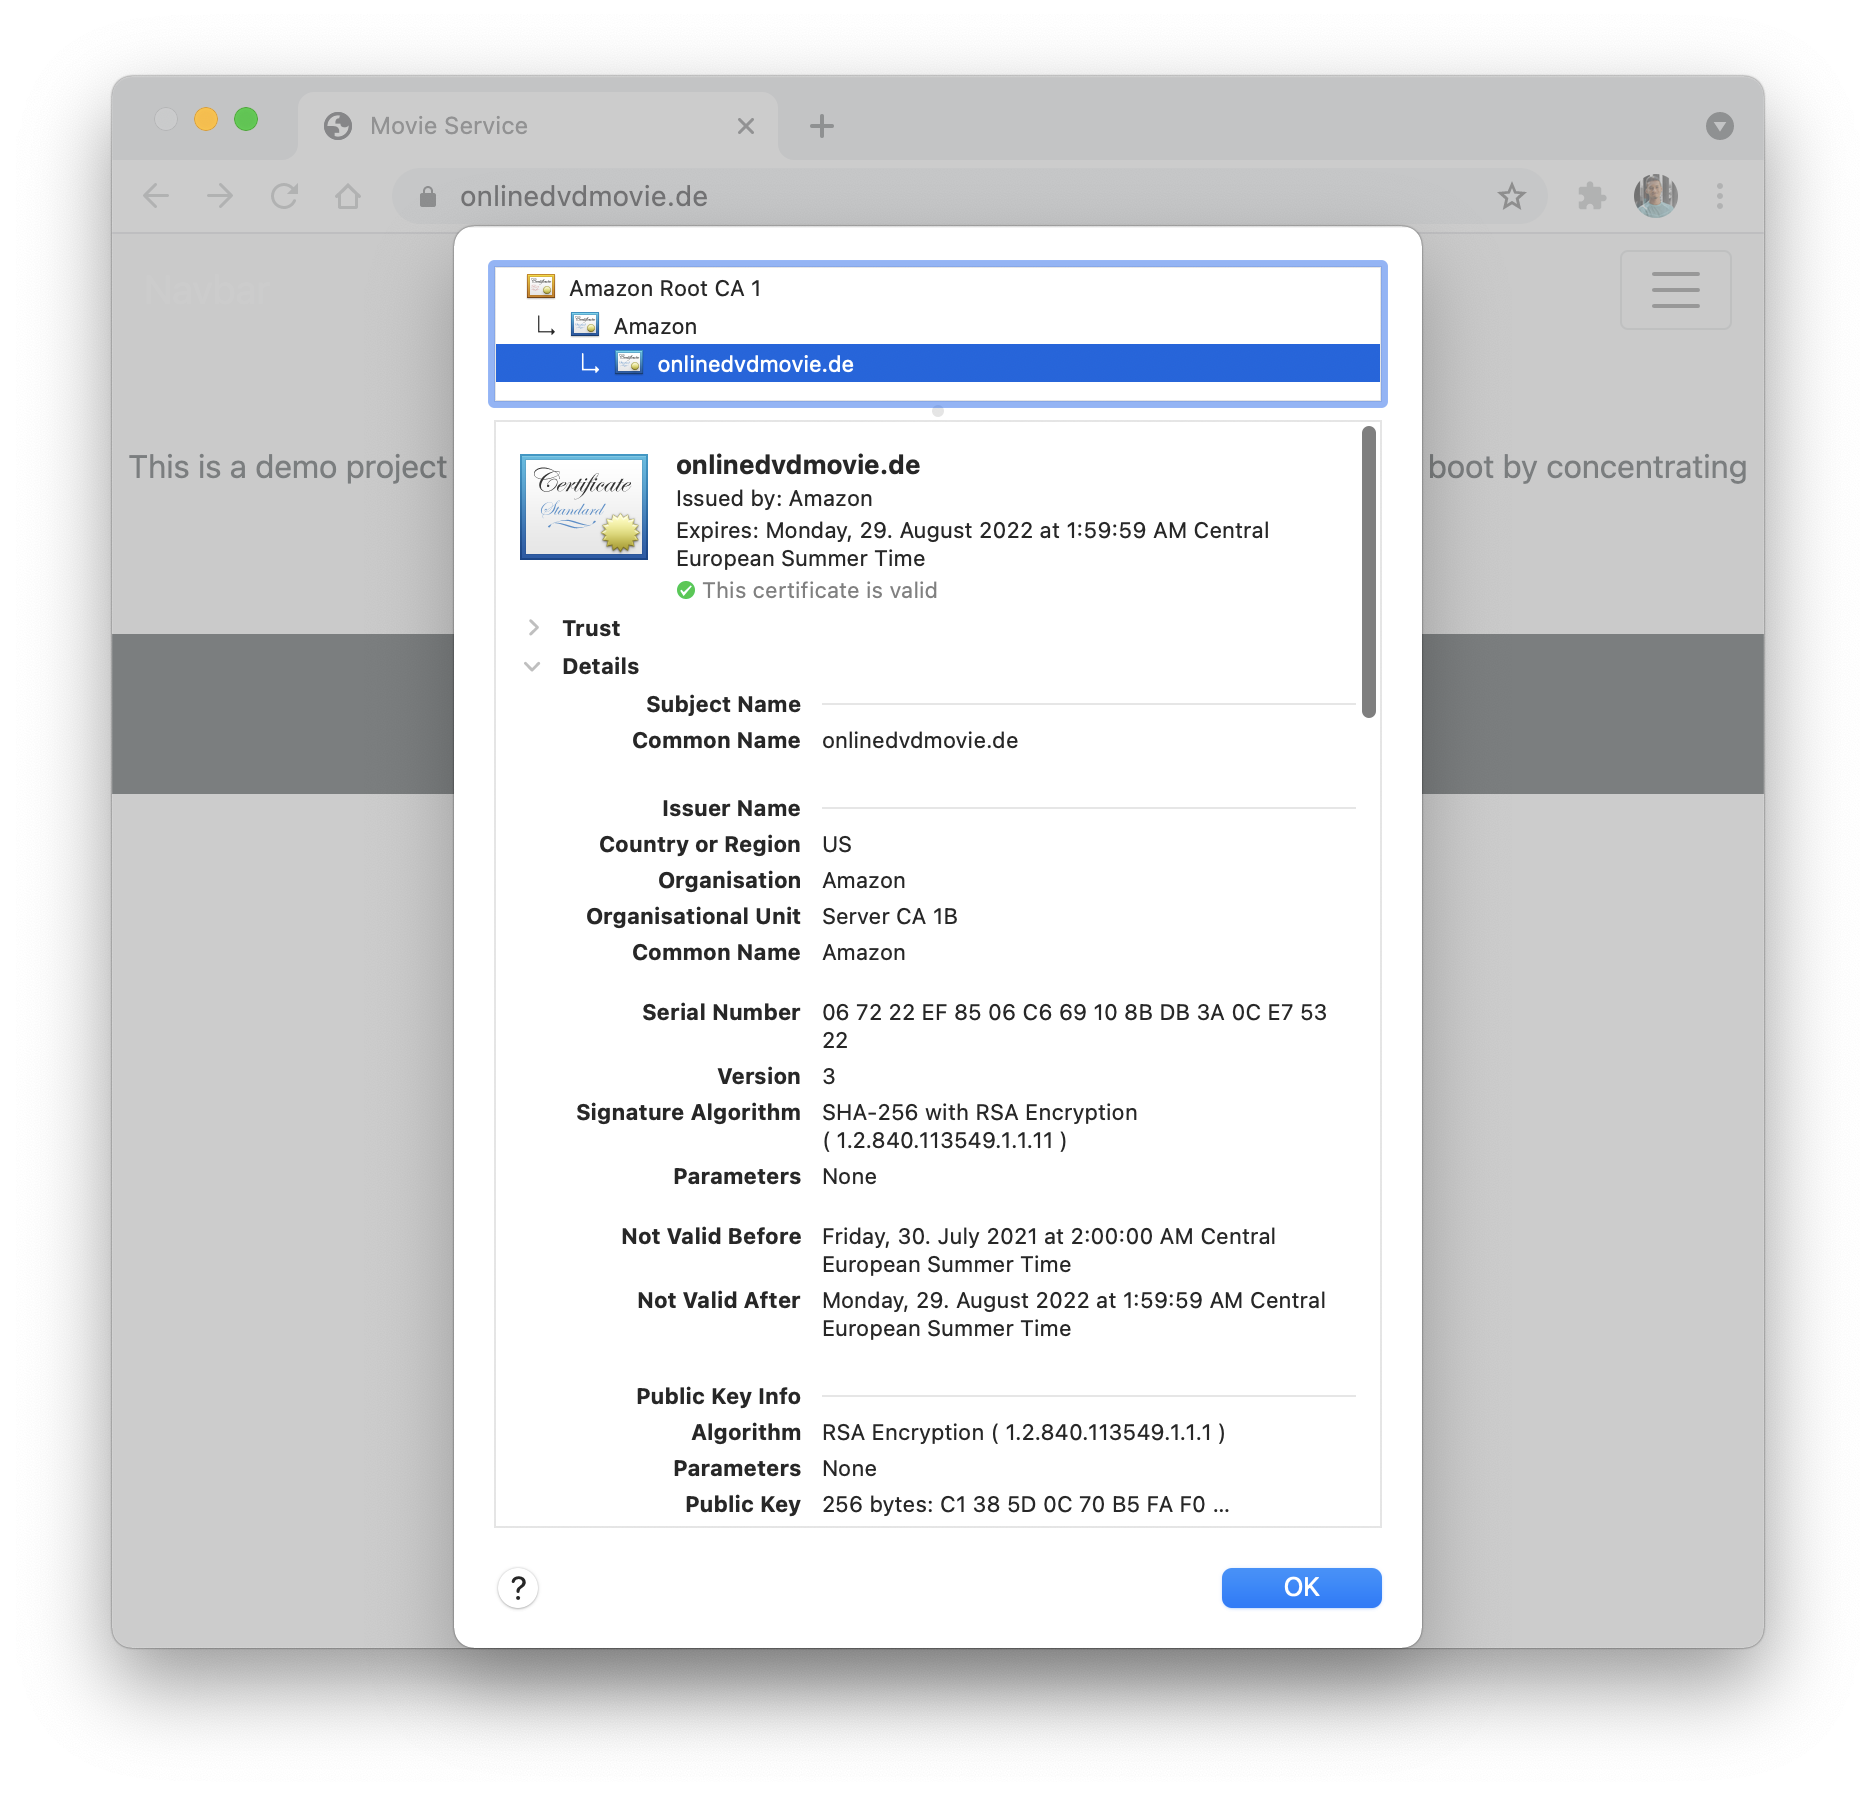
\includegraphics[scale=.36]{images/Sinchan/5sinchan.png}}
\caption{Certificate associated to the domain 'www.onlinedvdmovie.de'}
\label{fig5sinchan}
\end{figure}

We can verify that our application data is encrypted using the Wireshark application. When we analyze the captured packets in FIGURE, we can see that the first application data sent after the TLS handshake process (‘Client hello’ and ‘Server hello’) is encrypted. Further application data are using the TLS protocol of version 1.3, which verifies that the communication is encrypted.

\footnotetext{\href{https://www.wireshark.org}{Wireshark, Accessed 29.07.2021}}

\begin{figure}[h]
\centerline{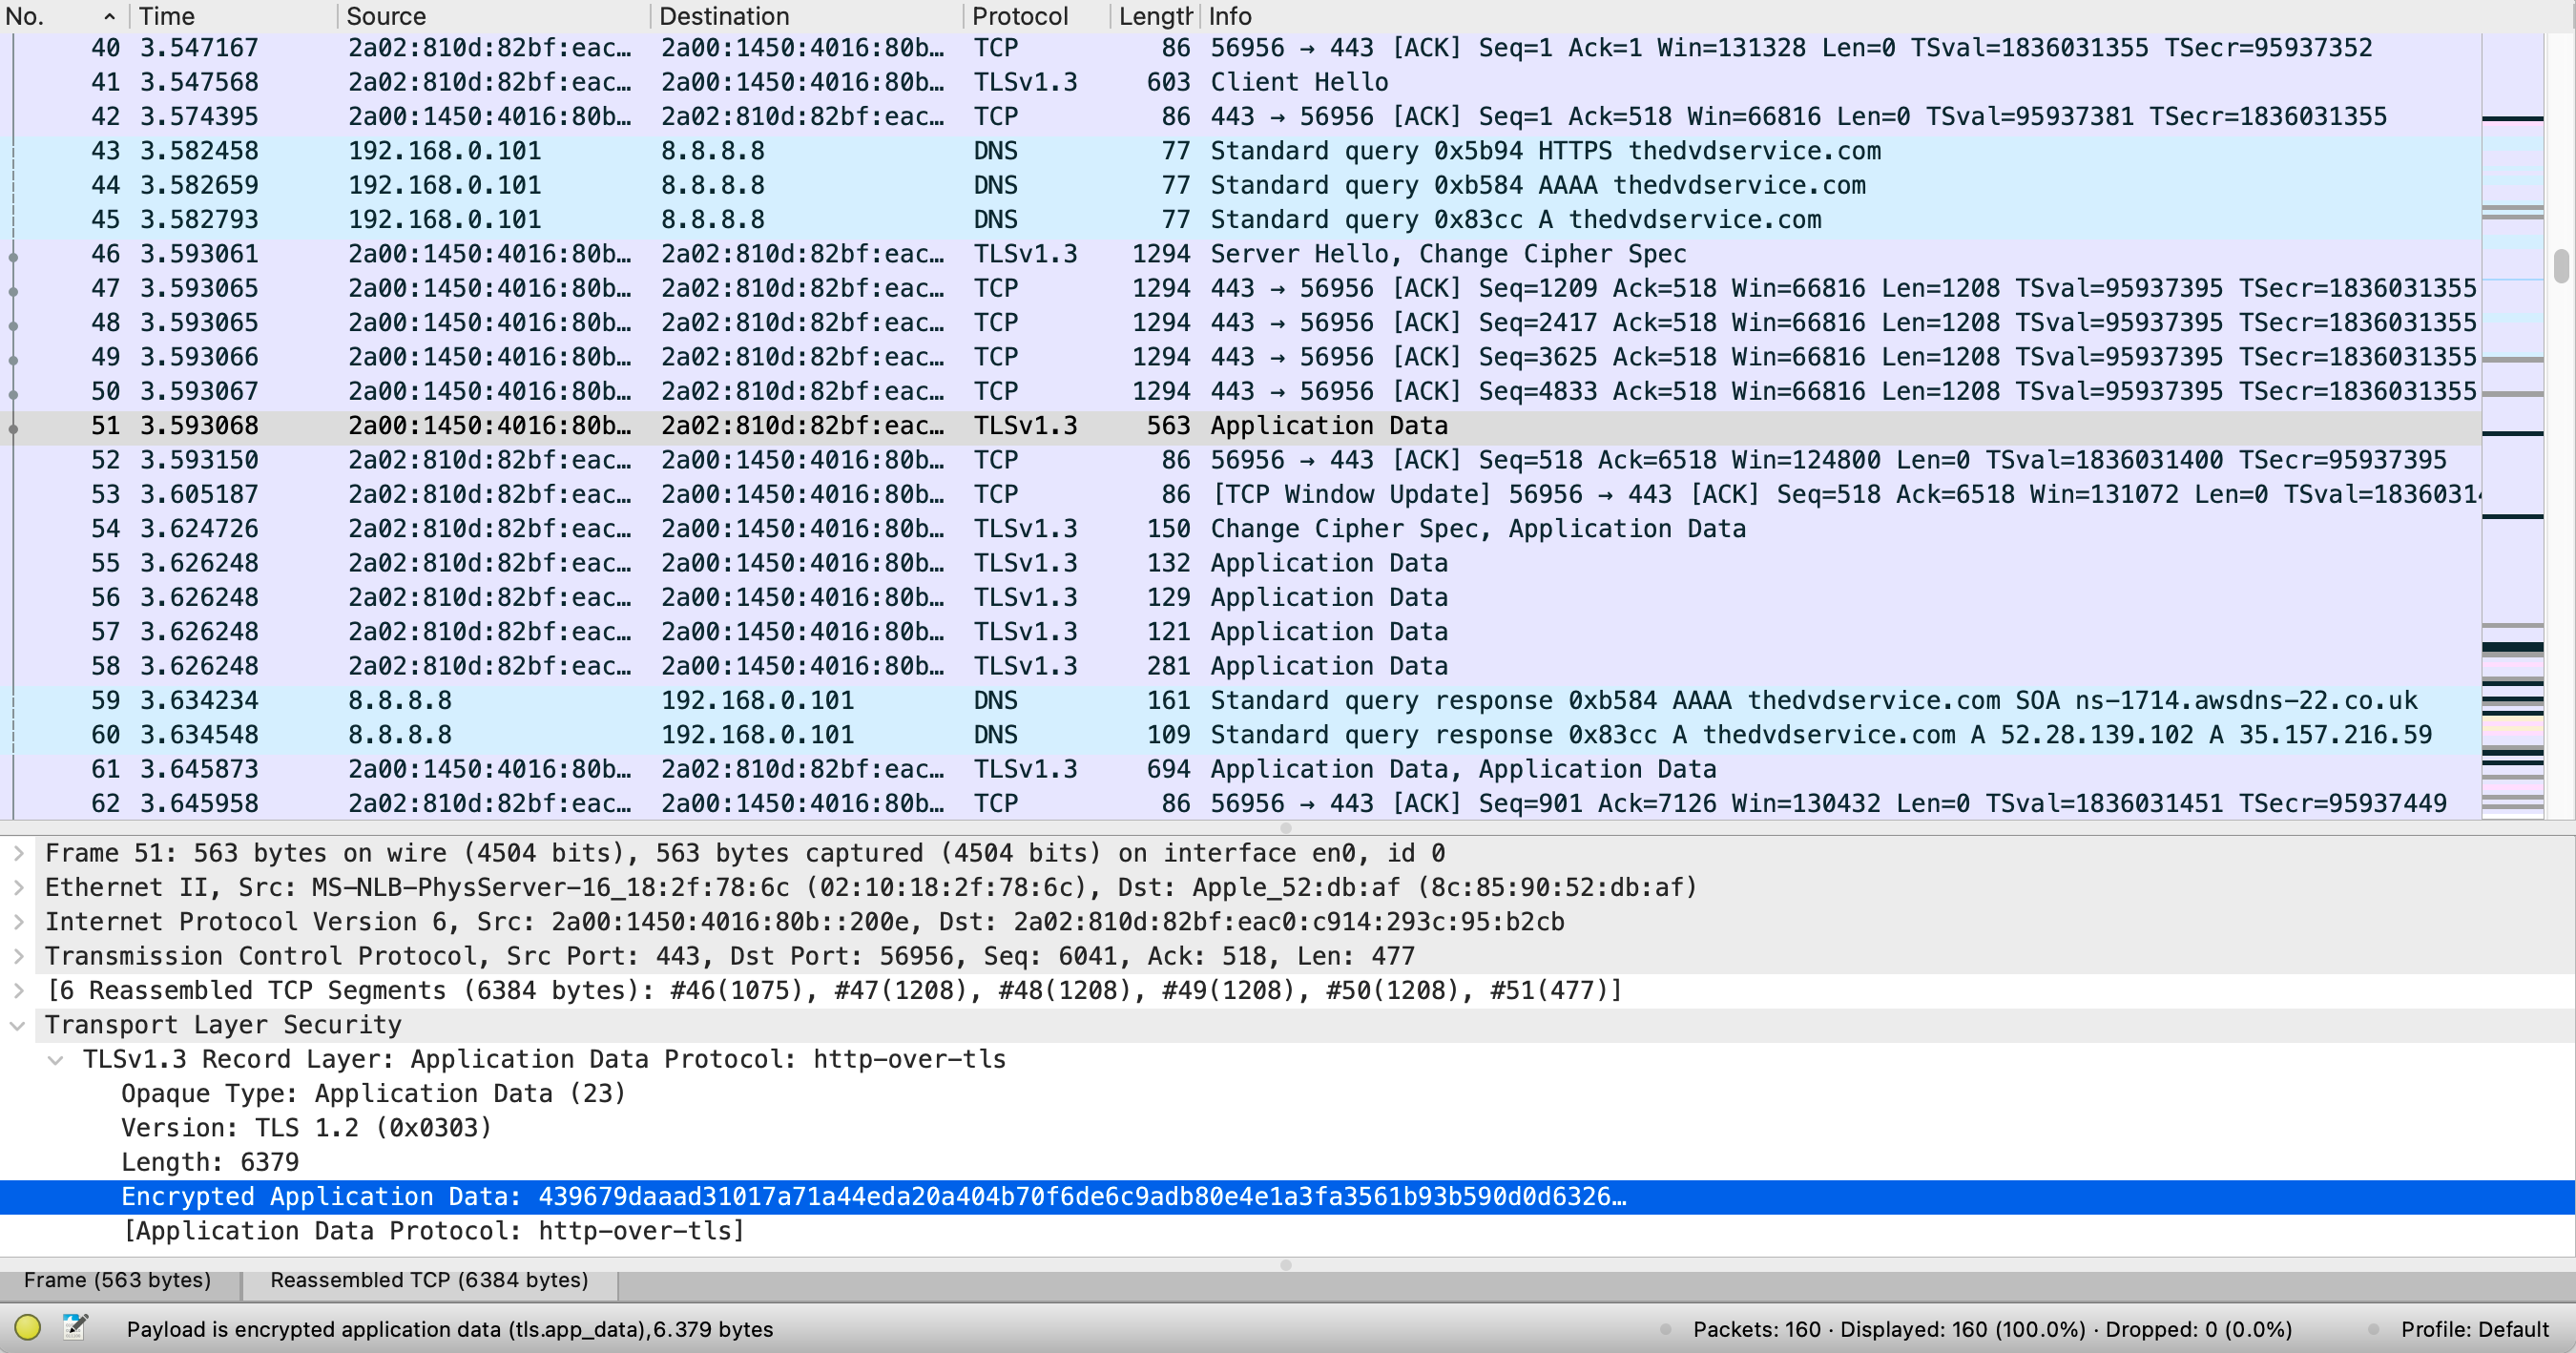
\includegraphics[scale=.36]{images/Sinchan/2sinchan.png}}
\caption{Wireshark capture for the traffic to domain 'www.onlinedvdmovie.de'}
\label{fig2sinchan}
\end{figure}




\subsection{Secure Database Access}

The database that we use for our application is PostgreSQL. AWS Relational Database Service (RDS) supports the PostgreSQL engine. With RDS, we can easily set up a database instance that helps in the easy scaling and management of PostgreSQL.

The AWS services reside in a Virtual Private Cloud (VPC). AWS VPC enables us to define a virtual network subnet. It allows us to run AWS services inside our defined VPC subnet. The major advantage of using such a private cloud is the ability to completely disable public accessibility.

\begin{figure}[h]
\centerline{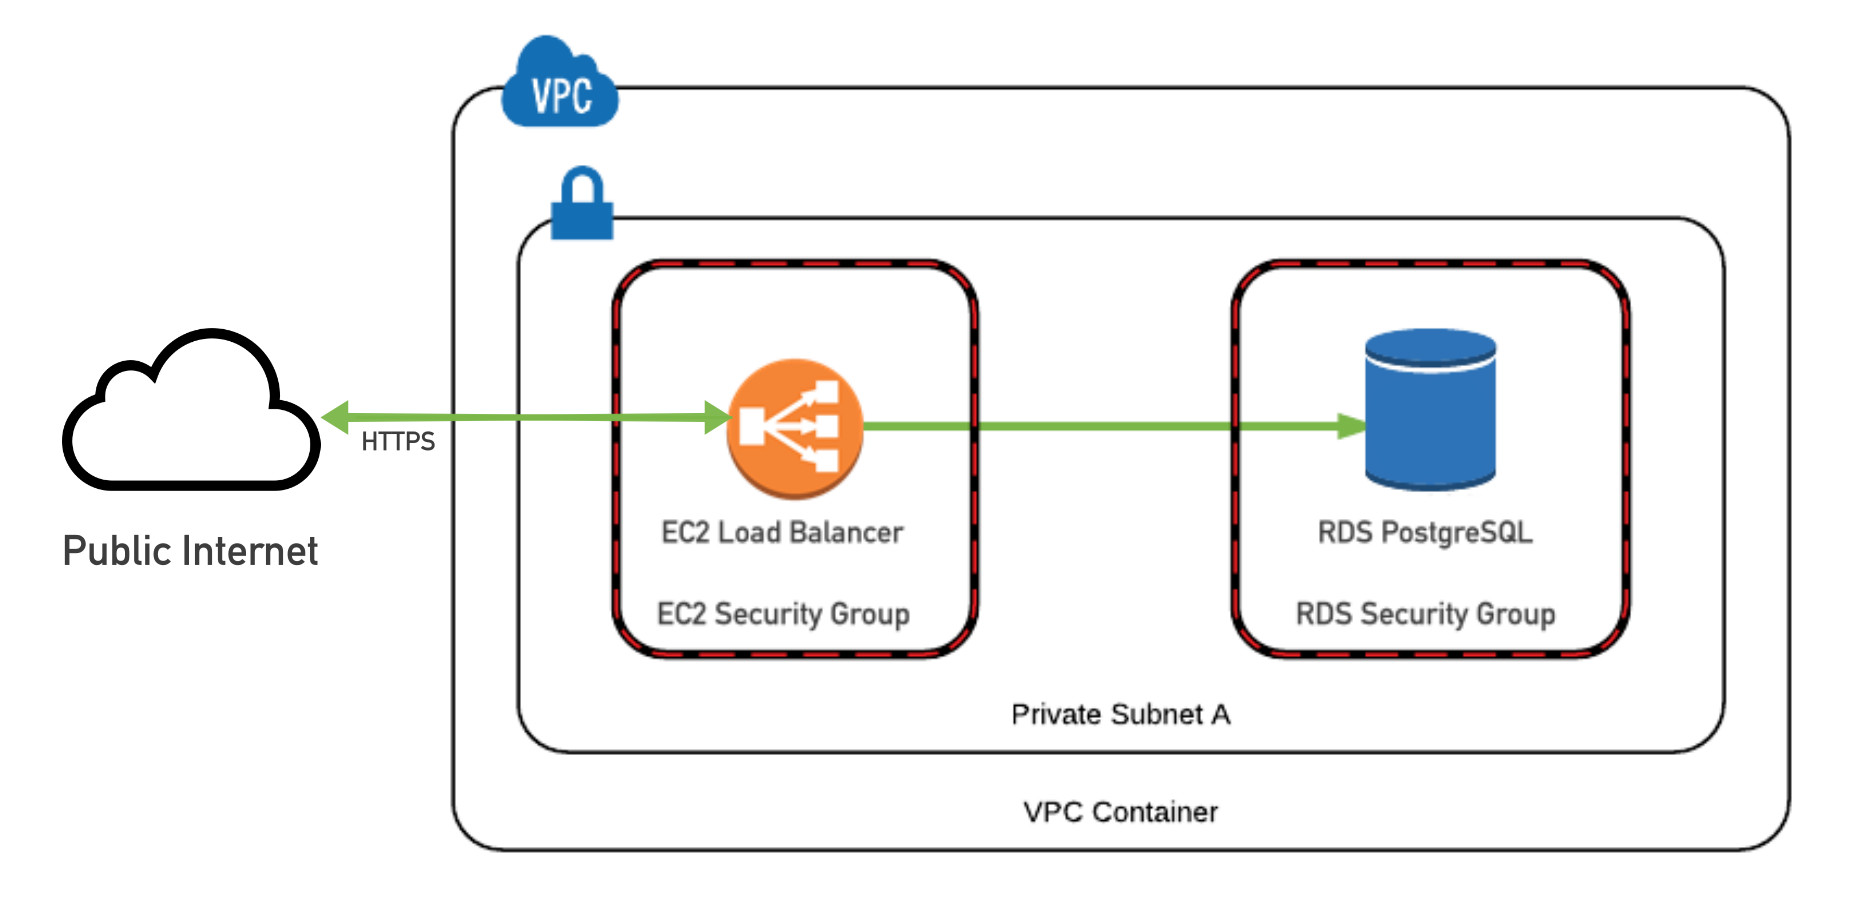
\includegraphics[scale=.36]{images/Sinchan/DB VPCsinchan.png}}
\caption{AWS VPC}
\label{DBVPC}
\end{figure}

Our application structure of access to the database is depicted in \autoref{DBVPC}. As the web application data is traversed through the Application Load Balancer over HTTPS and the internal communication is inside the VPC with no public accessibility, the access to the database is secured.

If there is a need to enable public accessibility for the database based on the use cases of the application, with AWS RDS, we can assign a certificate authority policy as well as the possibility to create proxies for the database instance.


\begin{figure}[h]
\centerline{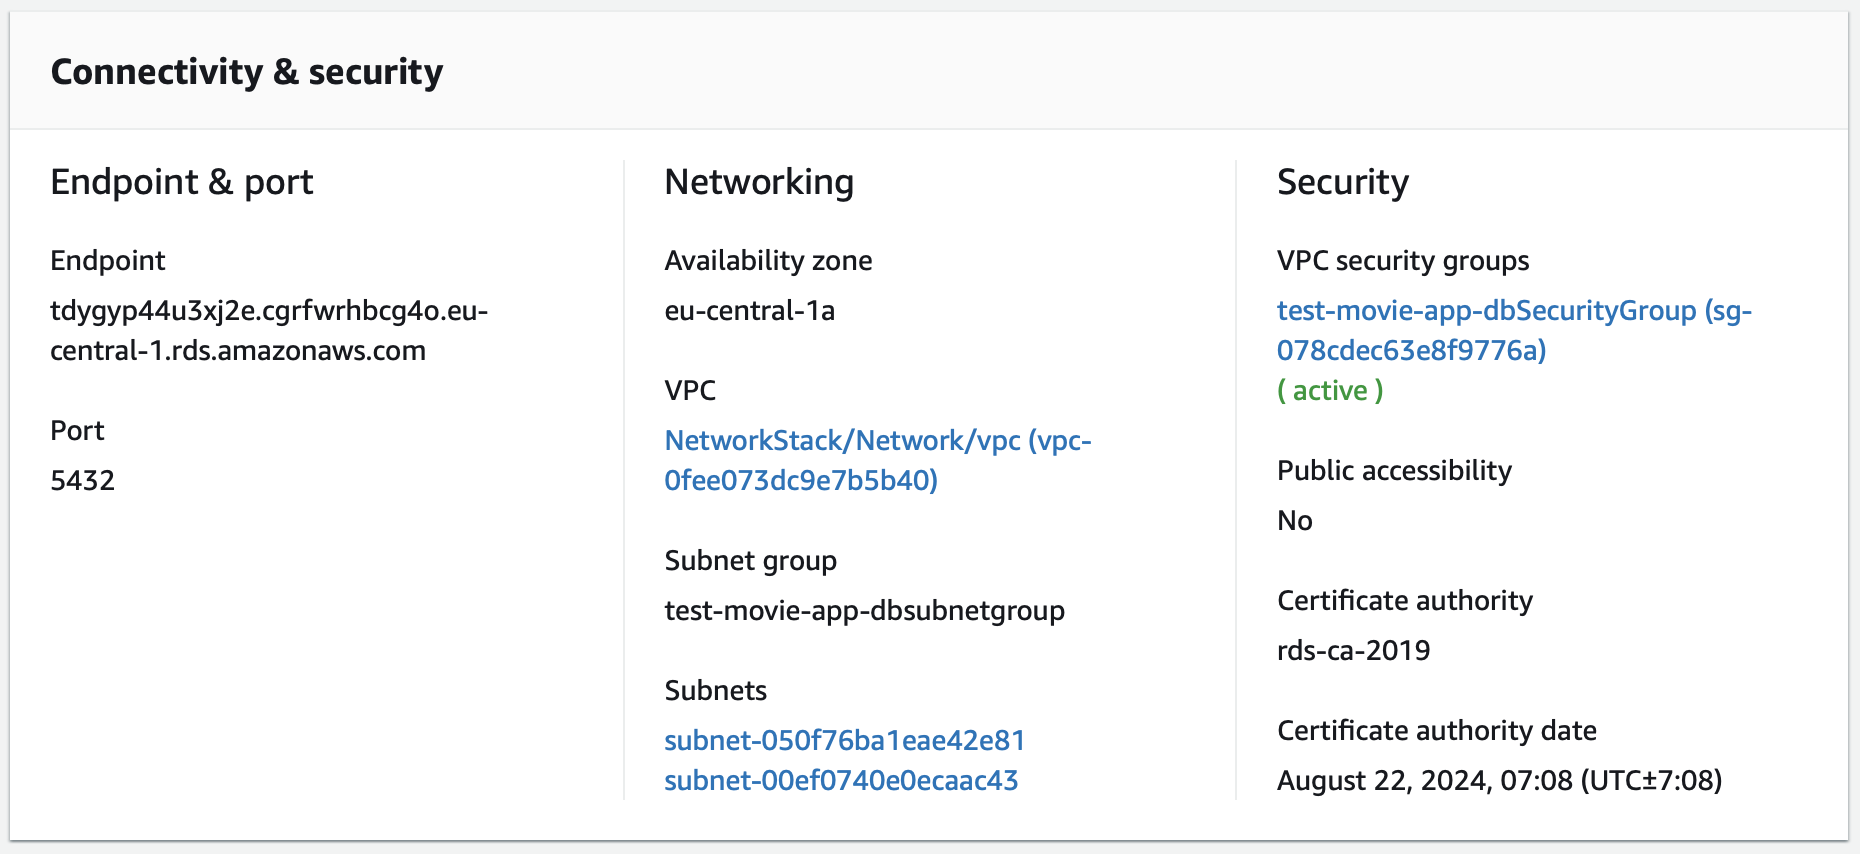
\includegraphics[scale=.36]{images/Sinchan/7sinchan.png}}
\caption{AWS VPC}
\label{fig7sinchan}
\end{figure}

\subsection{Secure Secret Management}

DevSecOps insists on the principle of not hard-coding user credentials or any secret inside the source code. It is essential to have a good secret management strategy. It is a vital part of securing the application. Unauthorized access to these secrets may compromise the security of the application.

AWS Secrets Manager allows us to store the secrets in a secure VPC, protected from unauthorized access. The Secrets Manager has the option to store credentials to the PostgreSQL as well as other API credentials. The secrets can be accessed by the application as a call to the Secrets Manager.

We can also set up the Secrets Manager to store other secrets and credentials as a key/value pair. These secrets are encrypted for further security. We encrypt secrets using either the default encryption key or can create our encryption key in the AWS Key Management Service (KMS) and use it for encryption. The default encryption key is not billed but the keys created in the AWS KMS are billed as per the usage of the corresponding keys.
